\chapter{Math: Abstract Algebra}\label{ch:group}
This chapter focuses on some of the abstractions in math, especially
as they apply to group theory. 
Groups appear often in physics:
Boosts and rotations in special relativity 
generate the Lorentz group, sets of gauge transformations equipped with 
function composition form gauge groups, etc. Some of this presentation
follows sections of Dummit and Foote~\cite{dummit_abstract_2004} and 
Georgi~\cite{georgi_lie_1999}.
In those presentations, the connection between groups and linear
transformations is emphasized; therefore we also include
some reminders of linear algebra.


\section{Preliminaries}


We want to discuss math in a fairly abstract way, in part because one of our
goals will be to look at generic mathematical structures. At the end of the book
we will look at groups, structures that have only three characteristics. We will
see that many math structures you've already encountered are examples of
groups
Hence we will need some notation that is agnostic to any particular math
structure.


To start, a {\it set}\index{set} is a collection of objects of
any kind, anything\footnote{This is technically wrong. It turns out that one has
to be very careful how a set is defined. Bertrand Russell was the first do
discover this; if you are interested in what can go wrong, look up
Russell's\index{Russell's paradox}
paradox. For our purposes, this subtlety won't matter.}
you can think of. We usually denote a set
with curly brackets
\begin{equation}
A=\{1,2,3,4\}.
\end{equation}
The things that the set contains are called {\it elements}\index{element}
or\index{member} {\it members}, and we indicate that, e.g. 1 is an element of
$A$ by writing
\begin{equation}
1\in A,
\end{equation}
which we read as ``1 is an element/member of the set $A$" or ``1 is in $A$".
If we want to refer to an arbitrary element $a$ of $A$, we write
\begin{equation}
a\in A,
\end{equation}
and if we want to say that $b$ is not a member of $A$, we write
\begin{equation}
b\notin A,
\end{equation}
The number of elements in a finite set is called its\index{cardinality}
{\it cardinality}. The cardinality of the set $A$ above is 4, and we write
\begin{equation}
  |A|=4.
\end{equation}
A {\it finite} set has a finite cardinality; otherwise it's an infinite set.


It is also useful to introduce an organizational hierarchy for sets. For
instance the set
\begin{equation}
  B=\{1,2,3,4,5,6\}
\end{equation}
is larger than $A$, but it contains $A$ entirely. We write
\begin{equation}
A\subset B.
\end{equation}
Talking about set logic is a good opportunity to introduce some more notation.
It is common to use $\Forall$ as shorthand for ``for all" or ``for any".
Since $A\subset B$, we know that $\Forall a\in A$ we must have $a\in B$.
To express that last idea, we write
\begin{equation}\label{eq:subsetIn}
a\in A\Rightarrow a\in B.
\end{equation}
The\index{set!empty} {\it empty set} $\emptyset$ is the set with nothing in it
at all. If a set has at least one element, it is\index{nonempty} {\it nonempty}.
From \equatref{eq:subsetIn} it follows that for any set $C$
\begin{equation}
\emptyset\subset C~~~~\text{and}~~~~C\subset C.
\end{equation}


A\index{function}
{\it function} or\index{map} {\it mapping} $f$ between $X$ and $Y$
associates $\Forall x\in X$ a unique element $f(x)\in Y$. We
write
\begin{equation}
f:X\to Y.
\end{equation}
Usually $X$ is called the\index{domain} {\it domain}
and $Y$ is called the\index{codomain} {\it codomain}.
The\index{image} {\it image} or\index{range} {\it range}
is $f(X)$, i.e. the set of all values $f$
maps to given the domain. Note $f(X)\subset Y$.

Next we classify a few different kinds of functions.
A function is\index{injection} {\it injective}
or\index{one-to-one} {\it one-to-one} if each element in $X$
maps to a different element in $Y$. We can express this symbolically as
\begin{equation}
 \Forall x_1,x_2\in X,~f(x_1)=f(x_2)\Rightarrow x_1=x_2.
\end{equation}
A\index{surjection} {\it surjective} or\index{onto} {\it onto} function
maps to every possible element of the codomain $Y$. Symbolically,
\begin{equation}
 \Forall y\in Y,~\Exists x\in X \suchthat y=f(x), 
\end{equation}
where we have introduced the symbol $\Exists$ as shorthand for ``there is at
least one" or ``there exists". Finally a function is\index{function!bijective}
{\it bijective} if it is both an injection and a surjection. In this case each
element of $X$ corresponds to exactly one element of $Y$, and vice-versa.
Pictorial representations of these kinds of functions are shown in
\figref{fig:mapping}.


\begin{figure}
\centering
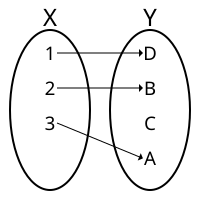
\includegraphics[width=0.45\linewidth]{figs/Injection.png}~~~
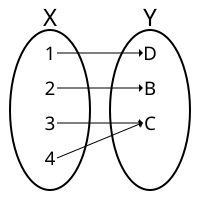
\includegraphics[width=0.45\linewidth]{figs/Surjection.png}\\
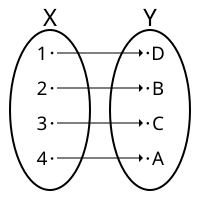
\includegraphics[width=0.45\linewidth]{figs/Bijection.png}~~~
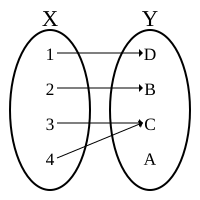
\includegraphics[width=0.45\linewidth]{figs/Not-Injection-Surjection.png}
\caption{Example mappings that are injective (top left), surjective (top right),
bijective (bottom left), and none of these (bottom right). Images taken from
Wikipedia~\cite{wiki:bijection}.}
\label{fig:mapping}
\end{figure}


To close out the section, we discuss a couple ways of putting sets together.
The most straightforward way is just to ``add" the sets, i.e. form a new set
whose elements include all the elements from the parent sets. For instance if
you have two sets $A$ and $B$, then the\index{union} {\it union} is
\begin{equation}
A\cup B = \{x\suchthat x\in A~\text{or}~x\in B\}.
\end{equation}
You can also create a set that contains only the elements that both $A$ and $B$ have
in common. This set is the\index{intersection} {\it intersection}
\begin{equation}
A\cap B = \{x\suchthat x\in A~\text{and}~x\in B\}.
\end{equation}
We exist in nature in a space of more than one dimension; therefore it is useful to be
able to combine sets into coordinates. We define the\index{Cartesian product}
{\it Cartesian product} of $A$ and $B$ as the set of tuples
\begin{equation}
A\times B=\{(a,b)\suchthat a\in A~\text{and}~b\in B\}.
\end{equation}


\section{Groups}\label{sec:gpprelim}


A {\it binary operation} \index{binary operation} $\bullet$ on a set 
$G$ is a function $\bullet : G\times G\to G$. A {\it group} \index{group}, 
then, is a set $G$ equipped with a binary operation $\bullet$ that satisfies 
the following axioms:
  \begin{enumerate}
    \item $\bullet$ is associative.
    \item $\Exists \id \in G$ such that $\Forall g \in G$, 
          \begin{equation}
            \id\bullet g=g\bullet \id=g. 
          \end{equation} This element $\id$ is called the {\it identity}.
          \index{identity}
    \item $\Forall g \in G\ \ \Exists g^{-1} \in G$, called the 
          {\it inverse} \index{inverse} of $g$, such that
          \begin{equation}
            g^{-1}\bullet g=g\bullet g^{-1}=\id.
          \end{equation}
  \end{enumerate}
If group elements commute under $\bullet$ the group is said to be 
{\it abelian} \index{abelian}. The {\it order} \index{order} of a group, 
denoted $|G|$, is the number of unique elements in the group\footnote{This
is at least true for finite groups.}. A {\it subgroup} \index{subgroup}
$H$ of $G$ is a non-empty subset of $G$ that itself forms a group under 
$\bullet$ and in this case we will write $H\leq G$. 
(It should be clear from context whether this symbol indicates group 
organization or magnitude.) Finally a group is {\it cyclic} \index{cyclic}
if it is generated by a single element; that is, if $\Exists g\in G$ such that 
$G=\{g^{n}\suchthat n\in\Z\}$.

It's actually not too common for mathematicians or physicists to write the
$\bullet$ explicitly when showing the composition of two elements. So for
example you will often see $gh$ as shorthand for $g\bullet h$. In general I will
only refer to operations on algebraic structures explicitly when giving the
definition of that structure. Therefore you can expect to see $gh$ instead of
$g\bullet h$ from here on out.

\begin{proposition}{}{}
  A subset H of G is a subgroup of G if and only if
  $$a,b\in H\Rightarrow ab^{-1}\in H$$
  \begin{proof}
    ($\Rightarrow$) Follows immediately from the definition of a subgroup. To 
    show ($\Leftarrow$) let $b\in H$. Then by the above conditional, $bb^{-1}
    \in H$, which shows $\id\in H$. To show the existence of inverses in $H$, 
    note $\id,b\in H\Rightarrow \id b^{-1}\in H\Rightarrow b^{-1}\in H$. 
    Finally, associativity is inherited from G.
  \end{proof}
\end{proposition}

An {\it equivalence relation} \index{equivalence relation} $\sim$ on a
set $G$ is a binary operation that has the following properties
$\Forall x,y,z\in G$:
\begin{enumerate}
  \item it is {\it reflexive}\index{reflexive}, i.e. $x\sim x$;
  \item it is {\it symmetric}\index{symmetric}, i.e.
        $x\sim y\Leftrightarrow y\sim x$; and
  \item it is {\it transitive}\index{transitive}, i.e. $x\sim y$ and
        $y\sim z$ $\Rightarrow$ $x\sim z$.
\end{enumerate}
Let $g\in G$. The set
\begin{equation}
\bar{g}\equiv\{x\in G\suchthat x\sim g\}
\end{equation}
is called an\index{equivalence class} 
{\it equivalence class}.


\begin{example*}{}{}
\begin{enumerate}
  \item $\Z,\ \Q,\ \R$, and $\C$ are all groups
        under addition, and
        \begin{equation}
          \Z \leq \Q \leq \R \leq \C.
        \end{equation}
        Each of these sets with 0 removed forms a group under
        multiplication. (We have to remove 0 because it has no multiplicative
        inverse.)
  \item Let $n\in \N$ and define an equivalence relation on 
        $\Z$ by 
        \begin{equation}
          a\equiv b\ (mod\ n)\ \Leftrightarrow\ n\ |\ (b-a).
        \end{equation}
        (We read this as ``$a$ is congruent to $b$ modulo $ n$" or ``$a$ is
        congruent to $b$ mod $n$.") Define an equivalence class by 
        \begin{equation}
          \bar{a}\coloneqq\{a+mn \suchthat m\in \Z\}.
        \end{equation}
        The set of all such equivalence classes is called {\it the integers 
        modulo n}\index{modular arithmetic} and is denoted by 
        $\Z/n\Z$ or $\Z_n$. It forms a group 
        under the ``addition" operation exemplified below. As a concrete 
        illustration, take $\Z_4$. It is of order 4, with 
        elements $\bar{0},\ \bar{1},\ \bar{2}$, and $\bar{3}$. To see how 
        addition works, note
        \begin{equation}
          \label{eq:chgtmaad1}
          \begin{aligned}
            \bar{1}+\bar{2}&=\{(1+2)+4(m_{1}+m_{2}) \suchthat m_{1},m_{2}
                             \in \Z\}\\
                         &=\{3+4m \suchthat m\in \Z\}\\
                         &=\bar{3}
          \end{aligned}
        \end{equation}
        and
        \begin{equation}
          \label{eq:chgtmaad2}
          \begin{aligned}
            \bar{3}+\bar{3}&=\{(3+3)+4(m_{3}+m_{4})\suchthat m_{3},m_{4}
                             \in \Z\}\\
                         &=\{2+4(1+m_{3}+m_{4})\suchthat m_{3},m_{4}
                             \in \Z\}\\
                         &=\{2+4m\suchthat m\in \Z\}\\
                         &=\bar{2}
          \end{aligned}
        \end{equation}
        It should be clear from the above that $\bar{0}$ is the identity
        element and $\Z_n$ is abelian and cyclic. I would
        also like to emphasize that the addition defined in 
        \equatref{eq:chgtmaad1} and \eqref{eq:chgtmaad2} is not the same
        addition as over the integers, even though I have chosen the same
        symbol for both cases. One should always be careful of what group
        operation is meant when the author is being lazy. 
  \item Sets of objects besides numbers also form groups. For example let $V$ 
        be any non-empty set of objects and let $S_{V}$ be the set of all
        permutations of $V$. Then $S_{V}$ forms a group under function
        composition called the {\it symmetric group}\index{group!symmetric} 
        on the set $V$.
\end{enumerate}
\end{example*}

In many situations, one encounters two groups of the same order that behave in
essentially the same ways. In a sense, one group is the same the original group,
masquerading about as a unique mathematical object. We could recover the
original group by merely relabeling elements of the masked group and viewing
its operation differently. Let us make these ideas more precise.
Let $G$ and $H$ be groups with operations $\bullet$ and
$\circ$, respectively. A map $\phi : G\to H$ satisfying
\begin{enumerate}
  \item $\phi(\id_G)=\id_H$ and
  \item $\phi(g \bullet h)=\phi(g)\circ\phi(h)$
\end{enumerate}
$\Forall g,h\in G$ is called a {\it homomorphism}.\index{homomorphism} 
If in addition to the above property we know that $\phi$ is a bijection, 
$\phi$ is said to be an {\it isomorphism} \index{isomorphism} of $G$ and 
$H$, we say that $G$ and $H$ are {\it isomorphic}, and we write $G\cong H$. 
Finally an {\it endomorphism}\index{endomorphism} is a homomorphism 
mapping a group to itself, and an {\it automorphism}\index{automorphism}
is a bijective endomorphism (isomorphism from a group to itself).

The above definition shows us that when $G\cong H$, $H$ is really just $G$ in
disguise. Since $\phi$ is a bijection we have a way of associating each element
of $H$ with exactly one element of $G$ and vice-versa (one could consider 
$\phi$ the relabeling), and the fact that $\phi$ is a homomorphism shows us
that the binary operations of the groups act the same way.

We note that if $G$ and $H$ are not isomorphic, it can be that $\phi$ maps
multiple elements of $G$ to the same element in $H$. The {\it
kernel}\index{kernel} of $\phi$, $\ker\phi$, is the set of elements in $G$ that map
to $\id_H$. 

A {\it field}\footnote{There are many instances where a term used in
a mathematical context is slightly different than its meaning in
a physics context. In a physics context, ``field" means something like
``a math object whose domain is every space-time point".
Due to these differing conventions, one usually has to determine based
on context which kind of field is meant.}\index{field} 
is a set $F$ equipped with two binary
  operations  $+$ and $\cdot$  satisfying the following properties:
  \begin{enumerate}
    \item $F$ equipped with $+$ is an abelian group. (Denote the 
          identity element with respect to this operation 0. 0 is often 
          referred to as the\index{identity!additive} {\it additive identity}.)
    \item $F-\{0\}$ equipped with $\cdot$ is an abelian group. (Denote the
          identity element with respect to this operation 1. As you may have
          guessed, 1 is called the\index{identity!multiplicative} 
          {\it multiplicative identity}.)
    \item $a\cdot (b+c)=(a\cdot b)+(a\cdot c)\ \ \Forall a,b,c\in F$. This is
          called the\index{distributive property} {\it distributive property}.
  \end{enumerate}
A {\it subfield}\index{subfield} 
is a subset $A$ of $F$ whose elements still form a field.
Later we will see that fields are the fundamental sets out of
which vectors are created.

\begin{example*}{}{}
\begin{enumerate}
  \item For any group $G$, $G\cong G$.
  \item The rotational symmetries of a regular $n$-gon are isomorphic to
        $\Z_n$.
  \item $\Q$ is a subfield of $\R$, which is in turn a subfield of $\C$.
\end{enumerate}
\end{example*}

\section{Quotient groups}\label{sec:q}\index{quotient group}

In this section we follow Ref.~\cite{dummit_abstract_2004}, which gives a nice
presentation of quotient groups. There, they point out that understanding
quotient groups more or less amounts to understanding group homomorphisms.

To begin we consider two groups $G$ and $H$ with a homomorphism $\phi:G\to H$.
The {\it fibers}\index{fiber} of $\phi$ are the sets of elements in $G$ mapping
to a single element in $H$, which is depicted graphically in
\figref{fig:quotientGroup}. If $a$ represents one of the dots in $H$,
the solid line above $a$ is the fiber of $\phi$ over $a$, which we can represent
at $\phi^{-1}(a)$.

Since $\phi$ is a homomorphism, it follows that however multiplication works 
among the dots in $H$, multiplication among the fibers must function the same
way. This suggests the creation of a new group, the {\it quotient group},
formed from the fibers. By construction, the quotient group with this
multiplication is clearly isomorphic to the image of $G$ under $\phi$.

\begin{figure}
  \centering
  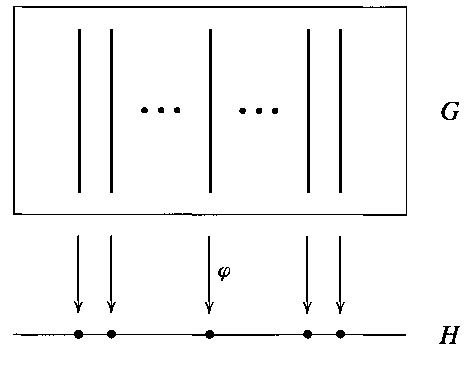
\includegraphics[width=0.60\linewidth]{figs/quotientGroup.pdf}
  \caption{Graphical depiction of constructing a quotient group from a group
$G$. The fibers, which are the solid, vertical lines, are mapped by the homomorphism 
$\phi$ into $H$. The set of fibers forms the quotient group. Image taken
from Ref.~\cite{dummit_abstract_2004}.}
  \label{fig:quotientGroup}
\end{figure}

Let $H\le G$ and $a\in G$. The {\it left coset} \index{coset} of $H$ with respect to 
$G$ is the set
\begin{equation}
   aH=\{ah\suchthat h\in H\}. 
\end{equation}
The {\it right coset} $Ha$ is defined similarly, but with $h$ and $a$
interchanged. You can think of e.g. a left coset of $H$ as a left translate of
$H$ by $a$, and similarly for the right coset. Any element of a coset is
called a {\it representative} of the coset.


We are now going to see that cosets define equivalence classes. To begin with
let $H\le G$; $x,y\in H$; and define a binary relation\footnote{You can
heuristically think of this equation as the statement that if I go ``forward" by
$x$, then ``backward" by $y$, I remain in $H$.} $\sim$ by
\begin{equation}\label{eq:cosetEquivalence}
  x\sim y \Leftrightarrow xy^{-1}\in H.
\end{equation}
\begin{proposition}{}{}
  $\sim$ is an equivalence relation.
  \begin{proof}
    We just need to check that it satisfies all the defining properties.
    \begin{enumerate}
      \item $xx^{-1}=\id$ $\Rightarrow$ $x\sim x$.
      \item $x\sim y$ $\Rightarrow$ $xy^{-1}\in H$ $\Rightarrow$
            $(xy^{-1})^{-1}\in H$ $\Rightarrow$ $yx^{-1}\in H$
            since $H$ is a group, so its elements have inverses.
            Hence $y\sim x$.
      \item $x\sim y$ and $y\sim z$ $\Rightarrow$ $xy^{-1}\in H$ and
            $yz^{-1}\in H$. Then since $H$ is closed under multiplication,
            $xy^{-1}yz^{-1}=xz^{-1}\in H$ $\Rightarrow$ $x\sim z$.
    \end{enumerate}
  \end{proof}
\end{proposition}
According to definition~\eqref{eq:cosetEquivalence}, given $H$,
the equivalence classes of $G$ under $\sim$ are the sets
$A\subset G$ satisfying $xy^{-1}\in H$ $\Forall x,y\in A$. To see why this is
important, fix $a\in A$. Then $\Forall x\in A$,
\begin{equation}
  \begin{aligned}
    x\sim a &\Rightarrow xa^{-1}\in H \\
            &\Rightarrow xa^{-1}=h~\text{for some}~h\in H\\
            &\Rightarrow x=ha\\
            &\Rightarrow A\subset Ha.
  \end{aligned}
\end{equation}
In other words, the equivalence classes are the right cosets of $H$! If we
instead defined the equivalence relation by $x\sim y$ $\Leftrightarrow$
$x^{-1}y\in H$, we would have found the equivalence classes to be the left
cosets of $H$.

We can now construct our new group. The group is a collection of cosets, but
it only forms a group if the cosets are special. In particular,
a subgroup $N\le G$ is said to be {\it normal}\index{normal} if 
$\Forall g\in G,$ $gN=Ng$. In this case we write $N\unlhd G$. The 
{\it quotient group}\index{quotient group} $G/N$ is the set of all cosets of 
$N$. We define an operation on $G/N$ by
\begin{equation}
  (xN)(yN)=x(Ny)N=x(yN)N=(xy)(NN)=(xy)N.
\end{equation}
Hence we see why it was so crucial that the subgroup be normal: It allowed
us to move the $y$ past $N$ in the second step, thus guaranteeing $G/N$ is
closed under this operation.
\begin{proposition}{}{}
  $G/N$ forms a group under the above operation.
  \begin{proof}
    This is pretty clearly a group because $G$ is. The identity is $\id N$,
    and each $xN$ has inverse $x^{-1}N$
  \end{proof}

\end{proposition}
\begin{proposition}{}{}
  $G/N$ forms a partition of $G$.
  \begin{proof}
    Let $g\in G$. We have to check that (1) $g$ belongs to some coset of $N$,
    and further that (2) $g$ does not belong to two different cosets.
    \begin{enumerate}
      \item Let $n\in N$ and define $g'=n^{-1}g$. Then
            $ng'=nn^{-1}g=g$, so $g\sim g'$.
      \item Let $x,y\in G$. If $g\sim x$ and $g\sim y$ then $x\sim y$ since
            $\sim$ is transitive. 
    \end{enumerate}
  \end{proof}
\end{proposition}
To summarize: If we find a normal subgroup $N$ of $G$, we can make a new group
$G/N$ by partitioning $G$ into disjoint cosets of $N$, which turn out to be
disjoint equivalence classes. These quotient groups are useful and pop up
pretty frequently; indeed the group $\Z/n\Z$, which we
encountered in the first section, is a quotient group. Now you understand the
notation.
\begin{example*}{}{}
\index{modular arithmetic}
  Take $G=(\Z,+)$ and $N=4\Z$. Clearly $4\Z$ is a
  normal subgroup of $\Z$ since it's commutative. To form the 
  quotient group $\Z_4=\Z/4\Z$, we find all cosets of $4\Z$.
  These are
  \begin{itemize}
    \item $4\Z$,
    \item $4\Z+1$=$\{4m+1\suchthat m\in\Z\}$,
    \item $4\Z+2$, and
    \item $4\Z+3$.
  \end{itemize}
  To check for instance that $4\Z+1$ is an equivalence class, we just
  need to show that $x,y\in4\Z+1\Rightarrow xy^{-1}\in4\Z$.
  Let $x=4m+1$ and $y=4n+1$ for some $m,n\in\Z$. Then
  $$xy^{-1}=x-y=4m+1-(4n+1)=4(m-n)\in4\Z.$$
  (This is an instance where the notation can be confusing; remember
  $\Z$ is being considered as a group under addition, so applying the
  inverse group operation means subtracting.) To see that there are no other
  cosets, note that $4\Z+4$=$4\Z$.
\end{example*}





\section{Vectors and vector spaces}\label{sec:vectors}

  This section begins a brief foray into linear algebra.
  Besides the fact that linear algebra has many applications to
  physics on its own, it is useful for understanding group
  representations, which we will discuss in \secref{sec:represent}.

  Let $F$ be a field. A {\it vector space}\index{vector!space} over $F$ is a set
  $V$ together with a binary operation $+$ under which $F$ is abelian and a
  mapping $F\times V\to V$, denoted $av\ \Forall a\in F$ and $v\in V$,
  satisfying
  \begin{enumerate}
    \item $(a+b)v=av+bv$,
    \item $(ab)v=a(bv)$,
    \item $a(v+w)=av+aw$, and
    \item $1v=v$
  \end{enumerate}
  $\Forall a,b\in F$ and $v,w\in V$. The elements $v$ and $w$ are\index{vector}
  called {\it vectors}\footnote{Note that within the contexts of high
  energy physics and relativity, the word ``vector" has a slightly more
  specific meaning: A ``vector" in those contexts is a vector in the
  mathematical sense along with a demand on how it behaves under
  Lorentz transformations.} A {\it subspace}\index{subspace}
  is a subset $W$ of
  $V$ that still forms a vector space over $F$. I will become immediately
  less formal and refer to the underlying field only if it's absolutely
  necessary.
  Let $V$ and $V'$ be vector spaces over a field $F$. A
  {\it linear transformation}\index{transformation!linear}
  of $V$ to $V'$ is a mapping $T : V\to V'$ such that
  \begin{enumerate}
    \item $T(v+w)=T(v)+T(w)$ and
    \item $T(av)=aT(v)$
  \end{enumerate}
  $\Forall a\in F$ and $v,w\in V$. We will often drop the parentheses
  and simply write $T(v)=Tv$. A linear transformation mapping a
  vector space to itself is called a {\it linear operator}.
  \index{operator!linear}\index{null space}\index{kernel}
  The {\it null space} or {\it kernel} of $T$ is
  \begin{equation}
    \mathcal{N}(T)\equiv\{v\in V:Tv=0\};
  \end{equation}
  i.e. it is the set of vectors annihilated by $T$. Finally $T$ is said
  to be {\it idempotent}\index{idempotent} if $T^2=T\neq\neq00$.
To connect some of the above definitions to what we learned in
\chref{ch:group}, we see that a linear operator is an endomorphism.
Furthermore we see that if a linear operator has an inverse, then it
is an automorphism.

  \index{function!distance}\index{metric}
  Let $M$ be some set. A {\it distance function} or {\it metric}
  is a function
  $d:M\times M\to \R$
  such that $\Forall x,y,z\in M$
  \begin{enumerate}
    \item $d(x,y)=0\Leftrightarrow x=y$,
    \item $d(x,y)=d(y,x)$,
    \index{triangle inequality}
    \item $d(x,z)\leq d(x,y)+d(y,z)$ (this is called the {\it triangle
          inequality}).
  \end{enumerate}
  \index{metric space}
  A {\it metric space}, then, is a set $M$ equipped with a metric $d$.
One can generalize the idea of a metric and relax some of these
conditions. I think for most purposes in physics this definition is sufficient.

\begin{example*}{}{}
 $\R^n$ forms a metric space when equipped with
  \begin{equation}
    d(x,y)=|x-y|=\sqrt{\sum\limits_{i=1}^n(x_i-y_i)^2}.
  \end{equation}
  \index{metric!Euclidean}
  This known as the {\it Euclidean metric}.
\end{example*}


Next we turn to the concepts of orthogonality and dimensionality, which
essentially tell us when two vectors are independent and how many independent
generators it takes to make a vector space.
We will formulate these ideas in terms of inner products.
  \index{product!inner}\index{product!scalar}
  Let $V$ be a vector space over $\C$. An {\it inner
  product} or {\it scalar product} is a mapping
  $(\ ,\ ):V\times V\to \C$
  satisfying $\Forall x,y,z\in V$ and $\alpha \in F$
  \begin{enumerate}
    \item $(x,y)=(y,x)^{*}$,
    \item $(x,y+z)=(x,y)+(x,z)$
    \item $(x,\alpha y)=\alpha(x,y)$
  \end{enumerate}
  Note that the above properties also imply $(x+y,z)=(x,z)+(y,z)$ and
  \index{vector!magnitude}\index{vector!norm}
  $(\alpha x,y)=\alpha^{*}(x,y)$. The {\it magnitude} or {\it norm}
  of a vector $x$ is $|x|\equiv(x,x)^{1/2}$. If $(x,y)=0$ then $x$
  \index{orthogonal}\index{orthonormal}
  and $y$ are said to be {\it orthogonal} and we write $x\perp y$.
  If in addition $|x|=|y|=1$, then they are {\it orthonormal}.

\begin{proposition}{}{orthog}
  Let $V$ be a vector space with inner product and let $W$ a subspace
  of $V$ with basis $\{w_1,...,w_N\}$. Consider the mapping $P:V\to W$
  defined by
  $$
    Pv=\sum_{i=1}^N\frac{(v,w_i)}{|w_i|^2}w_i.
  $$
  (This map is the {\it orthogonal
  projection}\index{orthogonal!projection}.)
  Then $v-Pv\perp W.$
  \begin{proof}
    We have
    \begin{equation*}
      \begin{aligned}
        (v-Pv,w_j)&=(v,w_j)-(Pv,w_j)\\
          &=(v,w_j)-\sum_{i=1}^N\frac{(v,w_i)}{|w_i|^2}(w_i,w_j)\\
          &=(v,w_j)-\frac{(v,w_j)}{|w_j|^2}|w_j|^2\\
          &=(v,w_j)-(v,w_j)\\
          &=0.
      \end{aligned}
    \end{equation*}
    Since $v-Pv$ is orthogonal to every basis vector of $W$, it is
    orthogonal to every vector in $W$.
  \end{proof}
\end{proposition}

The above proposition gives an algorithm to construct
a vector which is orthogonal to all elements in some subspace.
The algebra was a bit tedious but the intuition is clear:
if I project $v$ onto every basis vector of $W$ and add all
those contributions together, I get the part of $v$ that lies
within $W$. So I just subtract that away.

\section{Matrices}

Matrices play a fundamental role in physics as well.
We will see they are very useful for understanding different kinds of
symmetries, but they have many other applications.

Given a vector space $A^n$, we associate
$n\times n$ matrices\footnote{Such a matrix is usually called a {\it square
matrix}. Matrices don't have to be square matrices, i.e. they can have a
different number of rows than columns. In physics square
matrices matter the most, so that's all we will worry about for these notes.},
which have the form
\begin{equation}\label{eq:basicMatrix}
  M=\left(\begin{array}{cccc}
          a_{11}   & a_{12} &       & a_{1n}\\
          a_{21}   & a_{22} &       & a_{2n}\\
                   &        & \ddots&       \\
          a_{n1}   & a_{n2} &       & a_{nn}
            \end{array}\right). 
\end{equation}
We call each entry $a_{ij}\in A$, $1\leq i,j\leq n$, an {\it element}. The position
of each element is indicated by two subscripts, the left
indicating the row number and the right indicating the column number.


Matrices as defined above\footnote{That is, square matrices. By the way,
in this context of mapping vector spaces into themselves, we sometimes
call matrices {\it operators}\index{operator}.} map $A^n$ into itself, i.e.
\begin{equation}\label{eq:operatorDef}
  M:A^n\to A^n.
\end{equation}
In general, this mapping is achieved through matrix multiplication. If one
multiplies a vector $v$ with a matrix $M$, one gets for the $i\nth$ component
of the product $Mv$
\begin{equation}\label{eq:matTimesVec}
  (Mv)_i=\sum_{j=1}^n a_{ij}v_j,
\end{equation}
where $M$ is our matrix and $v$ is a vector.

Matrices can be added together element-wise.
Analogously as with many kinds of number systems, it is useful to introduce
in $n$ dimensions an additive identity\index{identity!additive} or zero matrix as
\begin{equation}
  \zd_n=\left(\begin{array}{cccc}
          0   & 0 &       & 0\\
          0   & 0 &       & 0\\
              &   & \ddots& \\
          0   &   &       & 0
            \end{array}\right), 
\end{equation}
i.e. it's the $n\times n$ matrix with 0 in every element. With our definition
of matrix addition, we find that for any $n\times n$ matrix $M$
\begin{equation}
\zd_n+M=M+\zd_n=M.
\end{equation}

Besides addition, it is useful to be able to carry out multiplication.
The simplest kind is scalar multiplication\index{multiplication!scalar},
which is defined similarly as with vectors.
One can also multiply a matrix $M$ and a matrix $L$. If $L$ has elements
$b_{ij}$, then the product $ML$ is defined element-wise by
\begin{equation}
  (ML)_{ij}=\sum_{k=1}^n a_{ik}b_{kj}.
\end{equation}
Notably, matrix multiplication is not in general commutative.
Again to continue our analogy with other number systems,
we introduce a multiplicative identity for matrices.
In $n$ dimensions, the {\it identity matrix} is
\begin{equation}
  \id_n=\left(\begin{array}{cccc}
          1   & 0 &       & 0\\
          0   & 1 &       & 0\\
          0   &   & \ddots& \\
          0   &   &       & 1
            \end{array}\right), 
\end{equation}
i.e. it is the matrix with 1 along the diagonal and 0 everywhere else. Using
matrix multiplication you can show that for any $n\times n$ matrix $M$
\begin{equation}
  M\id_n =\id_n M = M.
\end{equation}
Sometimes a matrix is {\it invertible}\index{matrix!invertible}, 
i.e. $\Exists M^{-1}$ so that
\begin{equation}
  M^{-1} M=\id_n. 
\end{equation}
If a matrix is not invertible, it is said to be 
{\it singular}\index{matrix!singular}.


To round out this discussion of thinking about matrices as math objects in their
own right, it is sometimes useful to define functions of matrices.
For starters, we can always
raise a matrix to an arbitrary power $k\in\N$. Hence we have well defined
functions of the form
\begin{equation}
f(M)=M^k\equiv\underbrace{M\,M\,...\,M}_{k\text{ times}},
\end{equation}
and as with ordinary numbers, we define $M^0\equiv \id_n$.
Using scalar multiplication and matrix addition, we are therefore also
able to sensibly define polynomials of matrices
\begin{equation}
f(M)=\alpha_0\id_n + \alpha_1 M + \alpha_2 M^2...+\alpha_n M^n.
\end{equation}
The fact that we can construct polynomials out of matrices empowers us
to define even more general functions through their Taylor series.
For example, the exponential $\exp:\R\to\R$ is given through its Taylor expansion
as
\begin{equation}
\exp(x)=\sum_{i=0}^\infty \frac{x^k}{k!}.
\end{equation}
This allows us to define the exponential of a matrix as
\begin{equation}\label{eq:expMat}
\exp(M)=\sum_{i=0}^\infty \frac{M^k}{k!}.
\end{equation}
All the typical elementary functions $\sin$, $\sinh$, and so on can be
analogously defined on matrices.
One can also do calculus on matrices:

\begin{proposition}{}{}
  Let $A$ and $B$ be $n\times n$ matrices with differentiable elements. Then
  $$
    \partial_\mu(AB)=(\partial_\mu A)B+A(\partial_\mu B).
  $$
  \begin{proof}
    We use the summation convention and abuse notation slightly: in the
    proposition statement $\partial_\mu$ has an identity matrix implicitly
    attached to it, but in this proof this symbol will also be used to
    denote the partial derivative operator applied to a single 
    element\footnote{I found notation like this to be extremely confusing
    when I was getting started. Sadly it very common notation, and as
    you can see, I have succumbed to this weakness myself.}. 
    Now since the matrix elements obey the product
    rule, we have
    \begin{equation*}
      \begin{aligned}
        \big(\partial_\mu(AB)\big)_{mk}
          &=\delta_{mn}\partial_\mu(A_{nl}B_{lk})\\
          &=\delta_{mn}\big(\partial_\mu(A_{nl})B_{lk}
                            +A_{nl}(\partial_\mu B_{lk})\big)\\
          &=\big((\partial_\mu A)B+A(\partial_\mu B)\big)_{mk}.
      \end{aligned}
    \end{equation*}
  \end{proof}
\end{proposition}


I am obligated to introduce some notation one frequently encounters
in physics with regard to matrices. The {\it trace}\index{trace} of an
$n\times n$ matrix is the sum of its diagonal elements,
\begin{equation}
  \tr M=\sum_i^nM_{ii}.
\end{equation}
When you {\it transpose}\index{transpose} a matrix, $M^t$, you interchange all of its
off-diagonal elements; i.e. the $i,j$-element gets replaced with the
$j,i$-element, and vice-versa.
The {\it complex conjugate}\index{complex conjugate}
of a matrix $M^*$ simply conjugates all its elements.
Finally we will sometimes need the conjugate-transpose or
{\it adjoint}\index{adjoint} of a matrix, which is indicated with a
little dagger\footnote{Hence we sometimes say ``$M$-dagger".},
$M^\dagger$. It is
\begin{equation}
M^\dagger\equiv (M^*)^t.
\end{equation}
The {\it determinant}\index{determinant}
of $M$ is 
\begin{equation}
  \det M\equiv\epsilon_{i_1...i_n}M_{1\,i_1}...M_{n\,i_n},
\end{equation}
where $\epsilon_{i_1...i_n}$ is the Levi-Civita symbol.
An important and often-used fact relating determinants
and inverses is the following:
\begin{proposition}{}{detSingular}
A matrix is invertible if and only if its determinant is nonzero.
\end{proposition}

Matrices will appear in many contexts for us, one of which
is quantum physics. Quantum physics was historically built up partially in
analogy to classical physics. As we were developing a consistent theory for these
small systems, we noticed that the kinds of relations we needed our observables
to obey could not be satisfied by familiar scalar fields like $\R$ and $\C$.
It was realized that we needed non-commutative symbols to understand,
for example, the famous Stern-Gerlach experiment. We already noted that matrix
multiplication is not commutative, so from that perspective matrices make good
candidates. More deeply, groups can be mapped into the set of
vector space automorphisms,
i.e. group elements can be 
represented\footnote{See \secref{sec:represent}.}\index{representation} by matrices,
and so we can always think of non-commutative symbols in terms of matrices,
whenever that helps us.

In the context of quantum physics, observables like position are represented by
matrices. But what we measure for an observable cannot depend on how we
represent\footnote{I mean ``represent" here in the colloquial sense.} it,
so we would like information about a matrix that is e.g. independent of
basis choice. The most important example of such information is as follows:
Let $V$ be a vector space $V$ over a field $F$ and let $v\in V$,
and suppose the matrix $M$ satisfies
\begin{equation}\label{eq:eigen}
Mv = \lambda v
\end{equation}
for some $\lambda\in F$. Then $v$ is an {\it eigenvector}\index{eigenvector} 
of $M$ with {\it eigenvalue}\index{eigenvalue} $\lambda$.

\begin{proposition}{}{eigenvalue}
  A matrix's eigenvalues don't depend on the basis. 
\end{proposition}

\propref{prp:eigenvalue} shows that eigenvalues are a great candidate
for measurable quantities, and indeed this is what we use in practice.
Finding eigenvectors and eigenvalues is pretty straightforward.
All eigenvalues of $M$ satisfy the
{\it characteristic polynomial}\index{characteristic polynomial}
\begin{equation}\label{eq:characteristicPolynomial}
\det\left(\lambda\id_n-M\right)=0,
\end{equation}
and in practice that's how one usually computes them.
Once you have found all the $\lambda$, you can plug them
into \equatref{eq:eigen} to find their corresponding
eigenvectors. If \equatref{eq:characteristicPolynomial}
has a root of order $m>1$, that eigenvalue is repeated.
Additionally, multiple vectors may have the same eigenvalue.
In case the eigenvalues are real, a matrix is
{\it positive definite}\index{positive definite} 
if its eigenvalues are all positive, and
{\it positive semidefinite}\index{positive semidefinite} 
if the eigenvalues are all nonnegative.

A matrix $U$ is said to be {\it unitary}\index{unitary} if
\begin{equation}\label{eq:unitary}
U^\dagger U=UU^\dagger=\id_n,
\end{equation}
i.e. unitary matrices are those whose inverses are the same as
their adjoints. Besides the fact that, by definition, these
matrices are easily invertible, they have the nice property 
for any vector $v$ that
\begin{equation}
|Uv|=\sqrt{(Uv,Uv)}=\sqrt{(Uv)^\dagger Uv}=\sqrt{v^2}=|v|,
\end{equation}
i.e. they preserve vector lengths. From
\equatref{eq:unitary} we see also they have determinant 1.
  A matrix $H$ is {\it hermitian}\index{hermitian}\footnote{Named
after a French mathematician, Charles Hermite. He's known
for a lot of stuff; for instance he was the first to
show that $e$ is transcendental.} if
\begin{equation}
H^\dagger=H. 
\end{equation}
Hermitian matrices by definition have real eigenvalues.
This is useful in the context of quantum physics, since physical observables
correspond to matrices, and eigenvalues of those matrices are measurable
quantities, which ought to be real.
Another nice property of hermitian matrices is the following:

\begin{theorem}{}{hermit}
  Hermitian matrices are diagonalizable.
\end{theorem}

A matrix $S$ is {\it symmetric}\index{symmetric} if
\begin{equation}
S^t=S,
\end{equation}
i.e. if the elements are symmetric about the diagonal.
Meanwhile a matrix $O$ is {\it orthogonal}\index{orthogonal} if 
\begin{equation}
O^tO=\id_n.
\end{equation}
This is
the real counterpart of a unitary matrix. 
\begin{proposition}{}{orthogonalMatrixLength}
Orthogonal matrices preserve length; i.e. if $O$ is
a real, orthogonal matrix and $v\in\R^n$, then 
$$
|Ov|=|v|.
$$
\end{proposition}

\subsection{General complex matrices}

Many of the matrices we deal with in physics are unitary, hermitian,
or orthogonal, and hence they have relatively nice properties.
Later in the context of lattice QCD, we will deal with more general
complex matrices that are not guaranteed to have these properties.
Therefore we collect here some useful results for complex matrices.

\index{Cayley-Hamilton theorem}
\begin{theorem}{The Cayley-Hamilton theorem}{cayleyHamilton}
Every square, complex matrix\footnote{Actually this theorem is
a bit more general as it applies to commutative rings.
But our matrices will always be over $\C$, so there is not
much point to introduce rings and make the distinction.} 
satisfies its own characteristic equation.
\end{theorem}

The Cayley-Hamilton theorem finds use as a method for
efficient computation of matrix inverses. For
example one can show for a $3\times 3$ matrix
\begin{equation}\label{eq:inv3x3CH}
M^3-(\tr M) M^2+\frac{1}{2}\left((\tr M)^2-\tr M^2\right) M
-\det M  \id_3=O.
\end{equation}
One can then multiply through by $M^{-1}$, and hence trade
the general problem of matrix inversion with a handful for matrix
multiplications, which may be faster.
Later we will encounter Lie groups whose representations
are traceless, which simplifies inverting such
matrices substantially.

\index{spectral theorem}
\begin{theorem}{Spectral theorem}{spectral}
Let $S$ be an $n\times n$ symmetric, complex matrix with
eigenvalues $\lambda_i$ and eigenvectors $u_i$. Then
We can decompose $S$ as
$$
S=U^t\Lambda U,
$$
where $\Lambda\equiv\diag\left(\lambda_1,...,\lambda_n\right)$ and
$U=\left(u_1,...,u_n\right)$.
\end{theorem}

The spectral theorem can be employed to find a useful
factorization for an arbitrary matrix, which goes by
the name of 
{\it singular value decomposition}\index{singular value decomposition} (SVD).
\begin{theorem}{Singular value decomposition}{SVD}
Any square\footnote{There is a statement also for non-square matrices.
But again, that's that not what we're interested in.}
matrix $M$ can be factorized as
$$
M=USV^t,
$$
where $S=\diag\left(s_1,...,s_n\right)$, $s_i\geq 0$,
and $U$ and $V$ are orthogonal matrices.
\end{theorem} 
SVD shows us that we can think of the action of any matrix on a real vector 
in three steps. More precisely, since $U$ and 
$V^t$ are orthogonal, they can be thought of
as rotations, and since $S$ is diagonal, it stretches each cardinal axis 
by $s_i$. These $s_i$ are called {\it singular values}\index{singular!value},
hence the name.

\begin{proposition}{}{semidefinite}
If $M$ is positive semidefinite, then its eigenvalues equal its singular values.
\end{proposition}

\propref{prp:semidefinite} is especially useful in the context of statistics,
since covariance matrices, discussed in \chref{ch:probability}, are
positive semidefinite. Hence SVD gives us a way to ``doctor" the eigenvalues
of a matrix, if we need to\footnote{For example in the context of statistics,
we need to invert covariance matrices, which turns out to be challenging if
the singular values span many orders of magnitude. 
We discuss in more detail in \secref{sec:numerics}.}. 

%Let A be a symmetric, positive definite matrix with singular value decomposition A=UΣVT (i.e. U, V are orthogonal matrices and Σ a diagonal matrix). Now look at how the singular values of A are related to the eigenvalues of ATA. Then think about how the eigenvalues of A are related to the eigenvalues of ATA and use that if A is symmetric, positive definite then its eigenvalues are real and positive.

We wrap up with a theorem that's useful to derive expressions relating
lattice interpolators and physical observables,
which we do in \secref{sec:QCDtherm}.
\begin{theorem}{The exp-trace-log (ETL) formula}{exptrlog}
  Let $M$ be an invertible, complex matrix. Then
  $$\det M = \exp \tr \log M$$
\end{theorem}
\index{ETL formula}


\subsection{Numerical considerations}\label{sec:numerics}


Many tasks in computational physics can be reduced to solving
$n$ simultaneous equations in $n$ variables. Collecting
the coefficients of the variables in a matrix $M$, this
can be expressed as
\begin{equation}\label{eq:solveGeneral}
Mx=b,
\end{equation}
where $b$ collects your RHS values and $x$ is the vector
of unknowns. Then \equatref{eq:solveGeneral} suggests a way
to find these unknowns:
\begin{equation}
x=M^{-1}b.
\end{equation}
Hence a situation where one has to determine some unknown
quantities subject to some constraints can always be cast
as the problem of inverting a matrix $M$, and it follows that
matrix inversion is crucial to scientific computing.

In an introductory linear algebra course,
one learns some standard techniques for inverting matrices,
usually Gauss-Jordan elimination. 
It's useful to use alternative algorithms whenever we can find them,
which may be faster or more numerically stable.
For instance, the Cayley-Hamilton theorem as applied
in \equatref{eq:inv3x3CH} is relatively fast.

Another consideration when inverting a matrix is numerical
stability. In particular, any algorithm that inverts a matrix is
limited by the machine's precision. So for instance if your
matrix has a near-zero determinant, then by
\propref{prp:detSingular}, you might intuit that while
formally invertible, computing this inverse is problematic,
since it's ``almost not invertible".

\thmref{thm:SVD} allows us some insight to such predicaments.
In particular we define the {\it condition number}\index{condition number}
$\kappa$ of a matrix $M$ to be the ratio of the largest
(in magnitude) singular value to the smallest, i.e.
\begin{equation}
\kappa(M)=\frac{\max\{s\}}{\min\{s\}}.
\end{equation}
$M$ is said to be {\it ill-conditioned}\index{ill-conditioned}
if $\kappa(M)$ is too large, i.e. if $1/\kappa(M)$ approaches
machine precision\footnote{Roughly less than $10^{-6}$ for
single precision and $10^{-12}$ for double.}.

One strategy to increase the stability of an inversion is to use
SVD to single out the problematic singular values of a matrix.
Then one can replace the smallest singular values with some small
number times the largest singular value, which then raises
the condition number by hand. This of course changes the matrix,
but in some circumstances, the change may be 
acceptable\footnote{For example in Ref.~\cite{dowdall_neutral_2019}
it is argued that such a modification, in their context applied
to a covariance matrix, serves to increase uncertainty estimates, which
they therefore argue is a conservative move.}.
A deeper discussion of SVD can be found in Ref.~\cite{press_numerical_2007}.


\section{Group representations}\label{sec:represent}



It turns out that many groups are isomorphic to sets of linear transformations
on vector spaces, and similarly that many sets of matrices equipped with matrix
multiplication form groups. In many cases these isomorphisms make dealing with
groups less abstract and more manageable; after all, everyone is comfortable
with matrices. In this section we will make these ideas precise, but we will
need to use linear algebra. 

The set of all automorphisms of a vector space $V$ is called
the {\it automorphism group}\index{group!automorphism} of $V$ or the 
{\it general linear group}\index{group!general linear} and is
denoted $GL(V)$. The set of all $n\times n$ matrices with entries from 
a field $F$ is called the {\it general linear group of degree $n$} and 
is denoted by $GL_{n}(F)$.
The reader may be concerned that the nomenclature
of the previous definition is poorly chosen. However if $V$ is a vector field
over the field $F$, the groups $GL(V)$ and $GL_{n}(F)$ are actually just two
ways of viewing the same thing. 

\begin{theorem}{}{}
  Let $V$ be an $n$-dimensional vector space over $F$. Then 
  $$GL(V)\cong GL_{n}(F).$$
\end{theorem}

Let $G$ be a group, $F$ a field, and $V$ a vector space over
$F$. A {\it linear representation}\index{representation} of $G$ 
is any homomorphism $D:G\to GL(V)$. A representation is said to be 
{\it faithful}\index{representation!faithful} if it is injective. 
The {\it dimension}\index{representation!dimension} of a representation 
is the dimension of $V$.

\begin{example*}{}{}
\leavevmode
\begin{enumerate}
  \item Every group has a {\it trivial}\index{representation!trivial} 
    representation, $D(g)=1$.
  \item 
  $\Z_3$ has a 1D representation
  \begin{equation}
    D\left(\bar{0}\right)=1,~~~~
    D\left(\bar{1}\right)=e^{2\pi i/3},~~~~
    D\left(\bar{2}\right)=e^{4\pi i/3}.
  \end{equation}
  In the original group addition modulo $n$ is the binary operation,
  while the representation takes ordinary multiplication on the reals.
  An example of a 3D representation of $\Z_3$ is
  \begin{equation}\label{eq:reg}
  \begin{gathered}
    D\left(\bar{0}\right)=\left(\begin{array}{ccc}
                           1 & 0 & 0 \\
                           0 & 1 & 0 \\
                           0 & 0 & 1
                          \end{array}\right),~~~~
    D\left(\bar{1}\right)=\left(\begin{array}{ccc}
                           0 & 0 & 1 \\
                           1 & 0 & 0 \\
                           0 & 1 & 0
                          \end{array}\right),\\
    D\left(\bar{2}\right)=\left(\begin{array}{ccc}
                           0 & 1 & 0 \\
                           0 & 0 & 1 \\
                           1 & 0 & 0
                          \end{array}\right).
  \end{gathered}
  \end{equation}
  \end{enumerate}
\end{example*}
The representation of \equatref{eq:reg} is constructed by 
the following general prescription. Take $V=\R^n$ 
and imagine that the group elements form an orthonormal 
basis; i.e. $\ket{e_i}=\ket{g_i}$. Now define
\begin{equation}
  D(g_1)\ket{g_2}=\ket{g_1g_2}.
\end{equation}
The dimension of this representation is clearly just the order
of the group. One can recover the matrix elements via
\begin{equation}
  [D(g)]_{ij}=\bra{e_i}D(g)\ket{e_j}.
\end{equation}
  This is called the {\it regular}\index{representation!regular} 
representation. Another advantage of using linear spaces to represent groups
is that we can make a change of basis for our convenience. You
will recall this is achieved by similarity transformations
of the form
\begin{equation}\label{eq:simtr}
  D(g)\to D'(g)=S^{-1}D(g)S.
\end{equation}
This transformation clearly preserves the group multiplication
rules because $S$ cancels with its inverse.

Let $D$ be a representation of $G$ over a vector space $V$ with
subspace $W$. $W$ is an {\it invariant subspace}\index{subspace!invariant} 
of $D$ if
$\forall w\in W$
\begin{equation}
  D(g)w\in W.
\end{equation}
If $D$ has an invariant subspace it is said to be {\it reducible};
\index{representation!reducible} otherwise it is {\it irreducible}. 
We will shorten irreducible representation as irrep. If two representations $D$
and $D'$ are related by \equatref{eq:simtr} they are {\it equivalent}.
\index{representation!equivalent}
If $D$ is equivalent to a representation whose matrix
elements are in block diagonal form
\begin{equation}
  D(g)=\left(\begin{array}{ccc}
             D_1(g) & 0      &       \\
             0      & D_2(g) &       \\
                    &        & \ddots
             \end{array}\right)
\end{equation}
where the $D_i$ are irreps, then $D$ is called {\it completely
reducible}. Sometimes this is written as
\begin{equation}
  D=D_1\oplus D_2\oplus ...
\end{equation}
and we say that $D$ is the {\it direct sum}\index{direct sum} 
of the representations $D_i$.

\begin{theorem}{}{}
  Every representation of a finite group is equivalent to a
  unitary transformation.
%  \begin{proof} 
%  Let $D$ be a representation of a finite group $G$. Define
%  $$
%    S\equiv\sum_{g\in G}D(g)^\dagger D(g).
%  $$
%  $S$ is clearly hermitian and positive semidefinite. By
%  Theorem~\ref{thm:hermit}, it is diagonalizable.
%  \end{proof}
\end{theorem}
\begin{theorem}{}{}
  Every representation of a finite group is completely reducible.
\end{theorem}

% Talk about simple, schur's lemma.

\section{Young tableaux}

Recall from \secref{sec:gpprelim} the permutation group on
$n$ objects, $S_n$. Any element in $S_n$ can be written
as a product of cycles, which are just cyclic permutations of subsets.
Conventional notation writes a cycle as a list of numbers between
parenthesis, indicating the set of elements are are permuted.
\begin{example*}{}{}
  Consider permutations of $V=\{x_1,...,x_n\}$. Then
  \begin{enumerate}
    \item (1) takes $x_1\to x_1$;
    \item (238) takes $x_2\to x_3\to x_8\to x_2$;
    \item a cycle of length $k$ is a {\it k-cycle};
    \item $\id$=(1)(2)...(n); and
    \item $(12)(3)...(n)\in S_n$ interchanges $x_1$ and $x_2$
          while leaving all other elements fixed.
  \end{enumerate}
\end{example*}
A simple $n$D representation of $S_n$ permutes the orthonormal
basis vectors of $\R^n$. If a permutation $\pi$ takes $x_i$
to $x_j$ then
\begin{equation}
  D(\pi)\ket{i}=\ket{j},
\end{equation}
which implies
\begin{equation}
  D(\pi)_{li}=\bra{l}D\ket{i}=\delta_{lj}.
\end{equation}
This is called the {\it defining representation}.
\index{representation!defining}

A set is called a {\it conjugacy class}\index{conjugacy class} if 
$gSg^{-1}=S$. If you have a group element $g_1$, the 
{\it conjugation} of $g_1$ is $gg_1g^{-1}$.
From the definition of normal subgroup in \secref{sec:q} we
see that normal subgroups are conjugacy classes. The conjugacy classes
of of permutations are just the cycle structure; for instance all
interchanges are in the same conjugacy class. One way of seeing this
is by looking at the defining representation. If you conjugate using
an interchange, all this does is switch the basis vectors
$\ket{i}$ and $\ket{j}$, which clearly has no impact on the cycle
structure. Then, since any permutation can be built from interchanges,
it follows that an arbitrary conjugation preserves the cycle
structure. 

\section{Lie algebras and Lie groups}

  A {\it Lie algebra}\index{algebra!Lie} is a vector space $L$ over a field $F$
  together with an operation $[\ ,\ ]:L\times L\to L$ called the 
  {\it Lie bracket}\index{Lie!bracket}that satisfies 
  $\Forall \alpha,\beta\in F$ 
  and $x,y,z\in L$
  \begin{enumerate}
    \item $[\alpha x+\beta y,z]=\alpha[x,z]+\beta[y,z]$ (the Lie bracket is 
          {\it bilinear}),
    \item $[x,x]=0$ ({\it alternating} on $L$), and
    \item $[x,[y,z]]+[z,[x,y]]+[y,[z,x]]=0$ (and satisfies the {\it Jacobi
          identity})\index{Jacobi identity}.
  \end{enumerate}
  The basis elements $T^a$ of $L$ are called the {\it generators}.
  \index{Lie!generator}

\begin{proposition}{}{}
  The Lie bracket is anticommutative.
  \begin{proof}
    $0=[x+y,x+y]=[x,x]+[x,y]+[y,x]+[y,y]=[x,y]+[y,x].$
  \end{proof}
\end{proposition}

Lie Algebras are used in physics to construct Lie groups.
Lie groups \index{group!Lie}are used to collect and analyze continuous symmetries of systems
and structures.
Let us see a way to construct Lie groups in physics. We will call the 
Lie group $G$, and the groups elements $g(\alpha)\in G$ will depend
smoothly on a set of continuous parameters $\alpha$. When we say ``smooth", we
mean that if two group elements are ``close together" in $G$, their parameters
are also close together. The identity is an important element in the group, so
we will parameterize elements with respect to it. We will shorthand
\begin{equation}
  \alpha=\left(\alpha^1,\,\alpha^2,\,...,\,\alpha^N\right),
\end{equation}
where $\alpha^a\in\R$. For our parameterization we set
\begin{equation}
  g(0)=\id.
\end{equation}
Then when we find a representation of the group, it will be
parameterized in the same way, so that
\begin{equation}
  D(0)=\id.
\end{equation}
In a neighborhood of $\id$ we can expand $D$. We find
\begin{equation}\label{eq:Depsilon}
  D(\epsilon\alpha)=\id+i\epsilon\alpha^aT^a+\order{\epsilon^2},
\end{equation}
where
\begin{equation}
  T^a\equiv-i\pdv{\alpha^a}D(\alpha)\Big|_{\alpha=0}.
\end{equation}
If we can identify the $T^a$ here with the Lie algebra $T^a$, we can see
how it Lie algebra generates the Lie group. The $i$ is included so that
if the representation is unitary, the $T^a$ are Hermitian.

We can move in a fixed direction away from the identity using
\equatref{eq:Depsilon} by simply raising it to some power. This suggests
defining the representation of the group elements as
\begin{equation}
  D(\alpha)=\lim_{k\to\infty}\left(1+i\alpha^aT^a/k\right)^k
           =\exp(i\alpha^aT^a).
\end{equation}
In the limit, this expression clearly goes to the representation of a group 
element, because $k$ becomes large, which means the term in parentheses is a 
group element, which means the whole product is a group element, since the
product of group elements stays in the group.

Since the exponentials are group elements, it must be that
\begin{equation}
  \exp(i\alpha^aT^a)\exp(i\beta^bT^b)=\exp(i\delta^cT^c)
\end{equation}
for some $\delta$. Since our parameterization is smooth, we can solve for
$\delta$ by Taylor expanding both sides. We write
\begin{equation}
  i\delta^cT^c=\log\big(1+\exp(i\alpha^aT^a)\exp(i\beta^bT^b)-1\big).
\end{equation}
Keeping terms up to only second order in $\alpha$ and $\beta$ we find
\begin{equation}
  i\delta^cT^c=i\alpha^aT^a+i\beta^bT^b-\frac{1}{2}[\alpha^aT^a,\beta^bT^b].
\end{equation}
We can rearrange the above to find
\begin{equation}
  [\alpha^aT^a,\beta^bT^b]=
   -2i(\delta^c-\alpha^c-\beta^c)T^c\equiv i\gamma^cT^c,
\end{equation}
where the bracket here denotes the ordinary commutator.
From the LHS of the above, we can see that the $\gamma^c$ must be some
sum of products of the $\alpha^a$ and $\beta^b$, so we can write
\begin{equation}\label{eq:gammac}
  \gamma^c=\alpha^a\beta^bf^{abc}
\end{equation}
for some constants $f^{abc}$. Hence
\begin{equation}\label{eq:liealg}
  [T^a,T^b]=if^{abc}T^c.
\end{equation}
The $f^{abc}$ are called the {\it structure constants}
\index{structure constants}. We have
\begin{equation}
  f^{abc}=-f^{bac}
\end{equation}
since $[A,B]=-[B,A]$. The structure constants essentially summarize the
group multiplication law. Sometimes we refer to the commutator relation
\eqref{eq:liealg} as the Lie algebra, which makes sense because it
essentially gives you a prescription for how the Lie bracket works.

Something worth noting is that we follow the same steps
as above to prove the Campbell-Baker-Hausdorff formula. In particular
if $X$ and $Y$ are non-commuting matrices, and $\epsilon$ is small,
we can expand
\begin{equation}
  \log\big(1+\exp(\epsilon X)\exp(\epsilon Y)-1\big)
\end{equation}
\index{Campbell-Baker-Hausdorff formula}
to second order in $\epsilon$ and then do some rearranging.
\begin{theorem}{Campbell-Baker-Hausdorff formula}{}
  $$
    \exp(\epsilon X)\exp(\epsilon Y)
      =\exp\left(\epsilon X+\epsilon Y+\frac{1}{2}[\epsilon X,\epsilon Y]
                           +\order{\epsilon^3}\right).
  $$
\end{theorem}

\subsection{SU(N)}

The Lie groups $\SU(2)$ and $\SU(3)$ are of considerable importance in the
Standard Model, as they used to describe weak and strong interactions.
General $\SU(N)$ is interesting for example
in the context of topological charge and for some grand unified theories.
Here we lay out some general properties of $\SU(N)$ matrices,
in the {\it defining representation}\index{representation!defining},
which is how they are commonly encountered.

In the defining representation, the generators $T^a$ are $N\times N$
traceless, complex, hermitian matrices, chosen so that
\begin{equation}
\tr T^a T^b=\frac{1}{2}\delta^{ab}.
\end{equation}
Of course, the generators will always obey \equatref{eq:liealg}.

It can be represented as
\begin{equation}
\SU(2)=\left\{
\left(\begin{array}{cc}
          a+ib   & -c+id  \\ 
          c+id   &  a-ib  \\
            \end{array}\right)\suchthat a,b,c,d\in\R \right\}.
\end{equation} 
That the matrix must have determinant 1 leads to the constraint
\begin{equation}
a^2+b^2+c^2+d^2=1,
\end{equation} 
which is the equation for the unit hypersphere in four dimensions, $S^3$. 

\begin{proposition}{}{}
  Let $A,B\in\SU(2)$ with parameterization
  $$
    A=a_0\id_2+i\vec{a}\cdot\vec{\sigma}, \qquad
    B=b_0\id_2+i\vec{b}\cdot\vec{\sigma},
  $$
  where the $\sigma_i$ are the usual Pauli matrices. Then
  \begin{equation*}
    AB=\id\left(a_0b_0-\sum\limits_{i=1}a_ib_i\right)
        +i\sum\limits_{i=1}\sigma_i\left(a_0b_i+a_ib_0
          -\sum\limits_{j\neq k}a_jb_k\epsilon_{jki}\right).
  \end{equation*}
  \begin{proof}
    \begin{equation*}
      \begin{aligned}
        AB&=\left(a_0\id+i\sum\limits_ia_i\sigma_i\right)
            \left(b_0\id+i\sum\limits_ib_i\sigma_i\right)\\
          &=\id\left(a_0b_0-\sum\limits_ia_ib_i\right)
            +i\sum\limits_i\sigma_i\left(a_0b_i+a_ib_0\right)
            -\sum\limits_{j\neq k}a_jb_k\sigma_j\sigma_k \\
          &=\id\left(a_0b_0-\sum\limits_ia_ib_i\right)
            +i\sum\limits_i\sigma_i\left(a_0b_i+a_ib_0\right)
            -i\sum\limits_i
                \sum\limits_{j\neq k}a_jb_k\epsilon_{jki}\sigma_i.
      \end{aligned}
    \end{equation*}
  \end{proof}
\end{proposition}
The parameterization of the above proposition exposes again
the bijection\footnote{Unfortunately this nice visualization
already breaks down for $\SU(3)$. I have read that it is ``the total space of 
an $S^3$ fibration over $S^5$. I don't really know what that means, but $S^3$
and $S^5$ are hyperspheres, so I sometimes think of an element in $\SU(3)$ being
characterized by two points, one on each hypersphere, with the hyperspheres
being somehow entangled.} between $\SU(2)$ and the three-sphere $S^3$.
In this parameterization, $a_\mu$ is a component of a 4D Euclidean vector where
$a_0\equiv a_4$. The vector, which specifies the $\SU(2)$ matrix entirely,
satisfies $a_\mu a_\mu=1$, which means it's a point on the surface of a 4D
hypersphere; i.e. the point is on $S^3$.
Additionally this parameterization is useful for carrying out
matrix multiplications on the computer.

\begin{proposition}{}{su2add}
  Let $A,B\in\SU(2)$. Then
  $$
  \frac{A+B}{\sqrt{\det(A+B)}}\in\SU(2).
  $$
  \begin{proof}
    Follows from $\det(cA)=c^n\det(A)$ for any $n\times n$ matrix $A$.
  \end{proof}
\end{proposition}

\subsection{Useful facts for Lie groups}

Here we collect some useful facts about common Lie groups that are encountered
in physics. Any time we give a dimension, it is over $\R$. 
That $G$ is a double cover of $H$ roughly means there are always two 
elements of $G$ corresponding to one element in
$H$. A summary of information is given in \tabref{tab:lie}.

The $\ON(1)$ isomorphism is very straightforward: In one spatial dimension, the
only isometry is a reflection.

To see the $\U(2)$ isomorphism, let $g\in\U(2)$, then show that
\begin{equation}
\sqrt{\det g\det g^*}=1.
\end{equation} 
The corresponding
$h\in U(1)\times SU(2)/\Z_2$ is given by
\begin{equation}
h=\left(\pm\sqrt{\det g},\pm\frac{g}{\sqrt{\det g}}\right),
\end{equation} 
where the sign reflects the $\Z_2$ part.

\begin{table}
\centering
\caption{Collection of properties of some Lie groups. }
\begin{tabularx}{\linewidth}{lCr}
\hline\hline
Group & Dimension & Notes\\
\hline
$\U(1)$  & 1          & $\cong S^1$ and $\SO(2)$\\
$\U(2)$  & 4          & $\cong \U(1)\times \SU(2)/\Z_2$\\
$\U(N)$  & $N^2$      & \\ 
$\SU(2)$ & 3          & $\cong S^3$, double cover of $\SO(3)$\\
$\SU(N)$ & $N^2-1$    & \\
$\ON(1)$ &            & $\cong\Z_2$, hence not Lie\\
$\ON(N)$ & $N(N-1)/2$ & $N>1$\\
$\SO(N)$ & $N(N-1)/2$ & \\
\hline\hline
\end{tabularx}
\label{tab:lie}
\end{table}


\bibliographystyle{unsrtnat}
\bibliography{bibliography}
 
